\chapter{Transizione di fase}
Generalmente transizioni di stato avvengono per $p$ e $T$ costanti, quindi la forma di energia pi\`u utile da considerare \`e l'energia libera di Gibbs
\[\Delta G=\Delta H-T\Delta S.\]
Poich\'e $dG=-SdT-Vdp$, si ha che se $p$ e $T$ restano costanti allora $\Delta G=0$, cio\`e \[T\Delta S=\Delta H.\]



\section{Transizione tra due fasi}
Chiamiamo le due fasi ``liquido" e ``vapore". 
\begin{notation}
Siano $n_L$ le moli di liquido e $n_V$ le moli di vapore.
\end{notation}
\begin{remark}[Energia libera di Gibbs molare]
Si ha che\footnote{nell'ultima uguaglianza abbiamo usato il fatto che l'energia \`e una grandezza estensiva.}
\[G=G_L(p_L,T_L,n_L)+G_V(p_V,T_V,n_V)\pasgnl={}n_Lg_L(p_L,T_L)+n_Vg_V(p_V,T_V)\]
dove $g$ \`e l'\textbf{energia libera di Gibbs molare}.
\end{remark}

\begin{remark}[Proporzione tra le fasi]
Per conservazione della materia $n_L+n_V=n$ \`e costante. Chiamiamo $\al$ la proporzione di liquido, cio\`e $n_L=\al n$ e $n_V=(1-\al)n$.
\end{remark}
\noindent
Possiamo riscrivere l'energia libera di Gibbs in termini di $n$ ed $\al$:
\[G=n\al g_L(p_L,T_L)+n(1-\al)g_V(p_V,T_V).\]
Poich\'e consideriamo tutto in regime di quasi-equilibrio, $T_L=T_V$ e $p_L=p_V$\footnote{le pressioni sono le stesse perch\'e c'\`e equilibrio meccanico.}. Abbiamo dunque ricavato che $G$ dipende solo da $p,\ T$ e $\al$.

\begin{proposition}[Condizione di equilibrio tra due fasi]
All'equilibrio si ha che
\[g_L=g_V.\]
\end{proposition}
\begin{proof}
Per $p$ e $T$ costanti sappiamo (\ref{GibbsDiminuiscePerPressioneETemperaturaCostanti}) che $\Delta G\leq 0$ , quindi siamo all'equilibrio solo se $G(\al)$ \`e minima, cio\`e\footnote{Per $p$ e $T$ costanti $G$ dipende solo da $\al$.}
\[0=\pp\al G=ng_L+0-n g_V\implies g_L=g_V.\]
\end{proof}

\subsection{Contenitore chiuso}
Modelliamo una contenitore chiuso ($U=cost$, $V=cost$).
\begin{notation}[Volume, energia interna ed entropia molari]
Scriviamo
\begin{align*}
V=&n\al v_L+n(1-\al)v_V\\
U=&n\al u_L+n(1-\al)u_V\\
S=&n\al s_L+n(1-\al)s_V
\end{align*}
\end{notation}
\begin{proposition}[Condizione di equilibrio tra due fasi]
All'equilibrio si ha che
\[g_L=g_V.\]
\end{proposition}
\begin{proof}
All'equilibrio $0=dV=dU=dS=dn$, quindi (ricordando che $p$ e $T$ sono costanti)
\begin{align*}
0=&dU+pdV-TdS=\\
=&d(n\al u_L+n(1-\al)u_V)+pd(n\al v_L+n(1-\al)v_V)-Td(n\al s_L+n(1-\al)s_V)=\\
=&n\al (du_L+pdv_L-Tds_L)+n(1-\al)(du_V+pdv_V-Tds_V)+\\
&+nd\al (u_L+pv_L-Ts_L)-nd\al (u_V+pv_V-Ts_V).
\end{align*}
All'equilibrio si ha che $du_L+pdv_L-Tds_L=0$ e similmente per il vapore, dunque
\[u_L+pv_L-Ts_L=u_V+pv_V-Ts_V.\]
Evidenziando le moli in questa equazione si ha
\[\under{=\frac{G_L}{n_L}}{\frac{U_L}{n_L}+p\frac{V_L}{n_L}-T\frac{S_L}{n_L}}=\under{=\frac{G_V}{n_V}}{\frac{U_V}{n_V}+p\frac{V_V}{n_V}-T\frac{S_V}{n_V}},\]
ovvero $g_L=g_V$ come volevasi dimostrare.
\end{proof}


\section{Caso generale}
Consideriamo $N$ componenti\footnote{moralmente $N$ \`e il numero di sostanze diverse} e $F$ fasi. Sia $n^{(i)}_k$ il numero di moli della componente $i$ nella fase $k$.\medskip

\noindent
Osserviamo che
\[G=\sum_{k\in\cpa{1,\cdots, F}}G_k(T,p,(n_k^{(i)})_{i\in\cpa{1,\cdots, N}}),\]
cio\`e a priori $G$ dipende da $NF+2$ variabili.

\begin{proposition}[Regola delle fasi di Gibbs]\label{RegolaFasiGibbs}
Il numero di gradi di libert\`a \`e
\[\boxed{\nu=2+N-F}\]
Questa \`e la \textbf{regola delle fasi (di Gibbs)}.
\end{proposition}
\begin{proof}
Consideriamo due fasi ($a$ e $b$) e la transizione dalla fase $a$ alla fase $b$:
\[\begin{cases}
n_a^{(i)}\to n_a^{(i)}-\delta n^{(i)}\\
n_b^{(i)}\to n_b^{(i)}-\delta n^{(i)}
\end{cases}.\]
Si ha che all'equilibrio
\[0=dG=dG_a+dG_b=\pp {n_a^{(i)}}{G_a}(-\delta n^{(i)})+\pp {n_b^{(i)}}{G_a}(\delta n^{(i)}),\]
ma l'energia libera di Gibbs \`e una grandezza estensiva, quindi vale la dipendeza lineare
\[\pp {n_k^{(i)}}{G_k}=\frac{G_k}{n_k^{(i)}},\]
segue dunque che
\[g_a^{(i)}=\frac{G_a}{n_a^{(i)}}=\frac{G_b}{n_b^{(i)}}=g_b^{(i)}.\]
Queste sono $F-1$ condizioni indipendenti per ogni componente.
\bigskip

\noindent Osserviamo inoltre che per ogni fase possiamo eliminare un grado di libert\`a considerando i rapporti tra le moli di componenti in quella fase.\bigskip

\noindent Tirando le somme si ha che i gradi di libert\`a sono
\[NF+2-(N(F-1)+F)=2+N-F.\]
\end{proof}



\begin{example}
Studiamo i valori di $N$, $F$ e $\nu$ per alcuni sistemi
\begin{itemize}
\item Fluido omogeneo: $N=1$, $F=1$, $\nu=2$
\item Fluido omogeneo dato da due gas: $N=2$, $F=1$, $\nu=3$
\item Acqua e vapore: $N=1$, $F=2$, $\nu=1$
\item Acqua, vapore e ghiaccio: $N=1$, $F=3$, $\nu=0$.
\end{itemize}
\end{example}

\begin{definition}[Punto triplo]
Considerando come sistema termodinamico l'acqua, esiste una precisa combinazione di temperatura e pressione tale per cui essa risulta in trasizione tra gli stati solido liquido e gassoso simultaneamente.\\
Questo stato si chiama \textbf{punto triplo} e i valori in questione sono una temperatura di $0.01 ^\circ \mathrm{C}$ e una pressione di $0.006\ \mathrm{atm}$.
\end{definition}

\newpage


\subsection{Grafici delle transizioni di fase}
Inseriamo qualche grafico che mostra come e quando le transizioni di stato avvengono:

\begin{figure}[!htb]
    \centering
    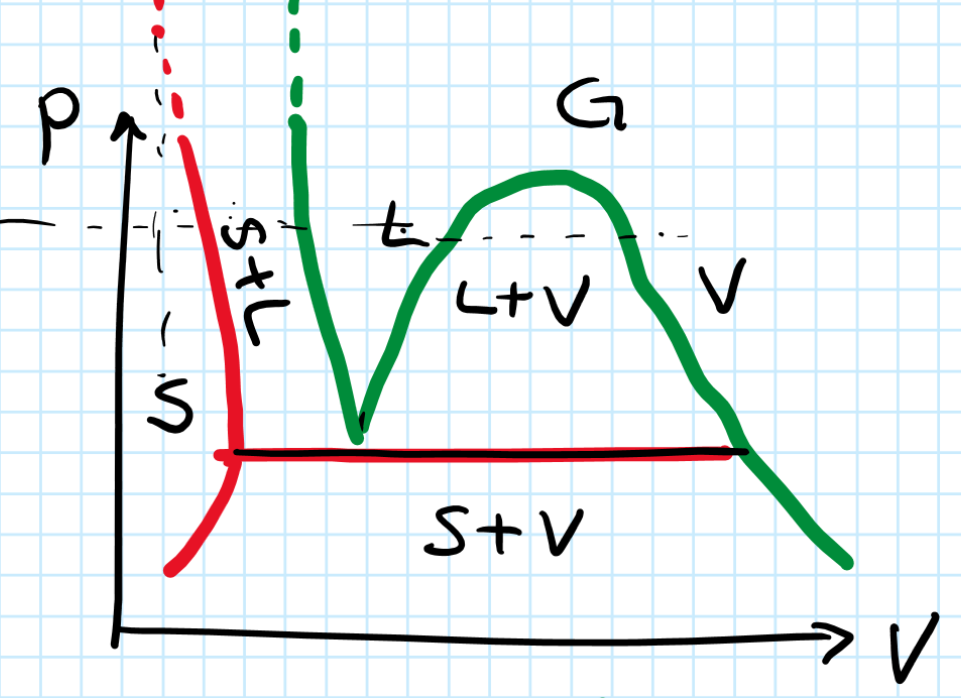
\includegraphics[width=7cm]{images/Grafico_p_V_transizione_di_stato.png}
\end{figure}

\begin{figure}[!htb]
    \centering
    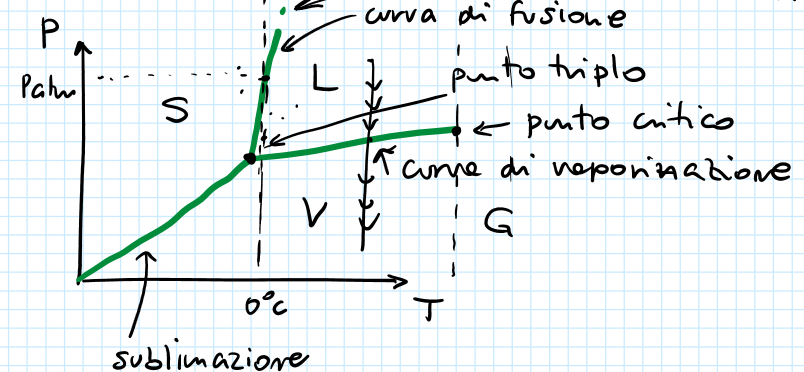
\includegraphics[width=11cm]{images/Grafico_p_T_transizione_stato.png}
\end{figure}


\subsection{Definizione di temperatura tramite gas}
L'esistenza del punto triplo ci permette di definire la temperatura in termini di una grandezza che possiamo misurare direttamente. 
\medskip

\noindent
A bassa pressione i gas tendono al regime di Gas ideale.\\
Se fissiamo il volume e le moli di gas possiamo definire $\theta$ in modo tale che $p=p_0(1+\al\theta)$, cio\`e poniamo 
\[\theta=\frac1\al\frac{p-p_0}{p_0}.\] 
Se imponiamo che l'acqua congeli per $\theta=0$ e evapori per $\theta=100$ allora ricaviamo $1/\al=273.15$. Notiamo inoltre\footnote{l'addizione di $\al\ii$ corrisponde alla traslazione che trasforma gradi Celsius in gradi Kelvin.}
\[\frac{p_2}{p_1}=\frac{\al\ii+\theta_2}{\al\ii +\theta_1}=\frac{\theta_2'}{\theta_1'}.\]
Possiamo dunque definire la temperatura (in Kelvin) come
\[T=\lim_{p^{(PT)}\to 0}273.16 \frac{p}{p^{(PT)}}\]
dove $p^{(PT)}$ \`e la pressione del gas nel termometro quando questo sistema \`e in equilibrio con il sistema di punto triplo con l'acqua. Il limite corrisponde a prendere gas sempre pi\`u rarefatti, cio\`e a lavorare nel limite dei gas perfetti dove vale la proporzionalit\`a sopra.
\medskip

\noindent Sfruttando questa definizione possiamo costruire un termometro a gas come in figura

\begin{figure}[!htb]
    \centering
    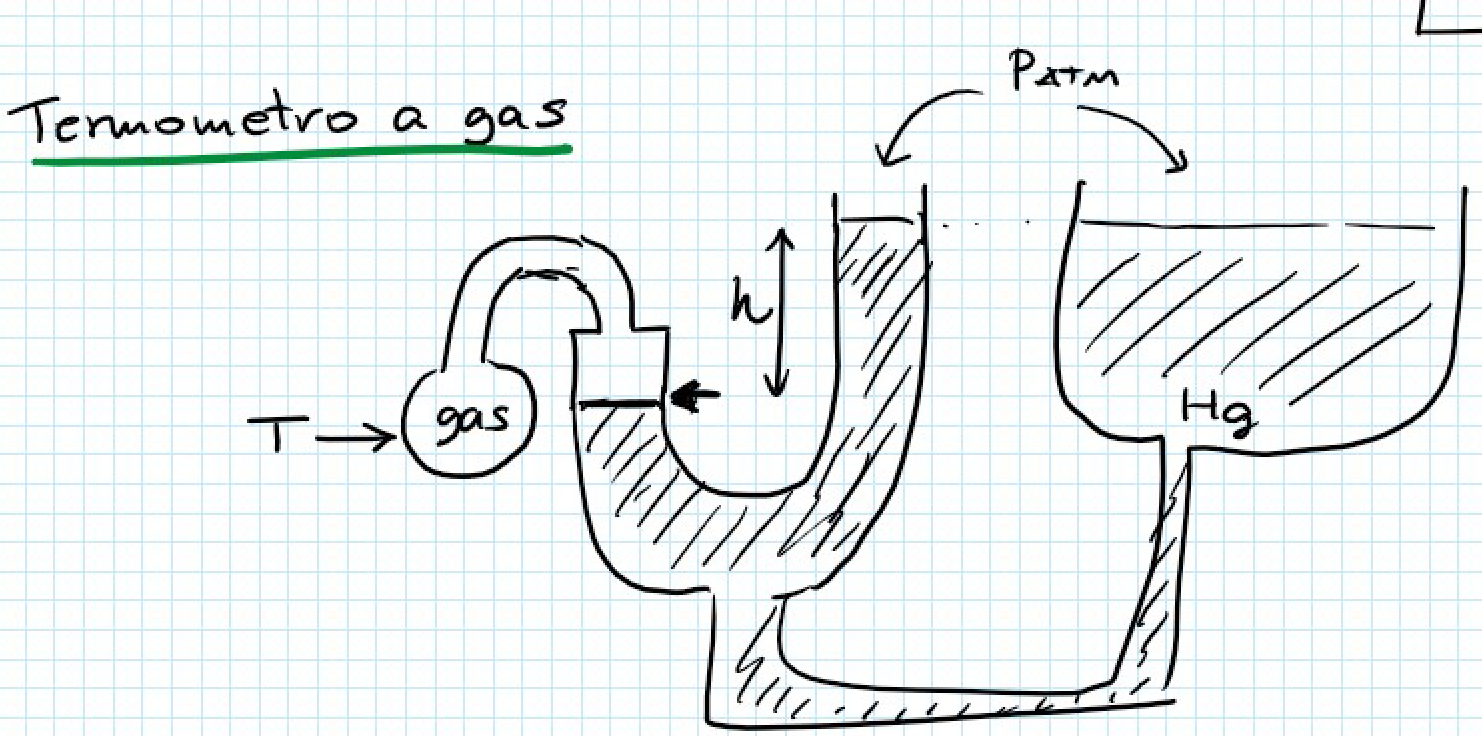
\includegraphics[width=11cm]{images/Termometro_a_gas.png}
\end{figure}


\noindent Quando il gas \`e alla temperatura che vogliamo misurare, misuriamo la differenza di altezza tra il livello a contatto con il gas e il livello di controllo posto a pressione atmosferica. 
Questa differenza \`e proporzionale alla differenza di pressione e questo ci permette di ricavare la temperatura se la fissiamo per quando \`e nel punto critico.




\section{Calore latente}
Consideriamo nuovamente il caso di due fasi (liquido e vapore). Osserviamo che fissata una temperatura, la pressione alla quale avviene la transizione di fase ne \`e una funzione. Segue che anche $V$ \`e una funzione di $T$.
\begin{remark}
Osserviamo che $dn_L=-dn_V$, quindi
\[\ppb VUT=\frac{u_V-u_L}{v_V-v_L}.\]
\end{remark}
\begin{proof}
Segue ricordando che $V=n_L v_L(T)+n_Vv_V(T)$ (e similmente per $U$) e che per le transizioni di fase $T$ \`e costante.
\end{proof}

\noindent
Per il primo principio
\[\delta Q=dU+pdV=dn_V(u_L-u_L+p(v_V-v_L)),\]
questo motiva la seguente
\begin{definition}[Calore latente]
Definiamo il \textbf{calore latente (molare) di vaporizzazione} come
\[\la=\frac{\delta Q}{dn_V}=u_V-u_L+p(v_V-v_L).\]
\end{definition}

\begin{proposition}[Equazione di Clapeyron]\label{EquazioneClapeyron}
Sulla transizione di fase
\[\dd Tp=\frac\la{T(v_V-v_L)}\]
\end{proposition}
\begin{proof}
Sviluppiamo $TdS$:
\[TdS=\under{=nc_V}{T\ppb TSVdT}+T\ppb VSTdV.\]
Applicando la relazione di Maxwell (\ref{RelazioniMaxwell}) data da $\ppb VST=\ppb TpV$ troviamo
\[TdS=nc_VdT+T\ppb TpVdV.\]
Combinando questo con $dU=TdS-pdV$ ricaviamo
\[dU=nc_VdT+\pa{T\ppb TpV-p}dV,\]
cio\`e
\[\ppb VUT=T\ppb TpV-p.\]
Ricordiamo ora che $\ppb VUT=\frac{u_V-u_L}{v_V-v_L}$, da cui
\[\frac\la{v_V-v_L}=T\ppb TpV,\]
che \`e la tesi se osserviamo che $\ppb TpV=\dd Tp$.
\end{proof}
\begin{remark}[Equazione di Clausius-Clapeyron]
Se $v_V\gg v_L$ allora per gas ideali
\[\dd Tp=\frac\la{RT^2}p\leadsto p\propto e^{-\la/RT}.\]
\end{remark}






